\begin{center}
	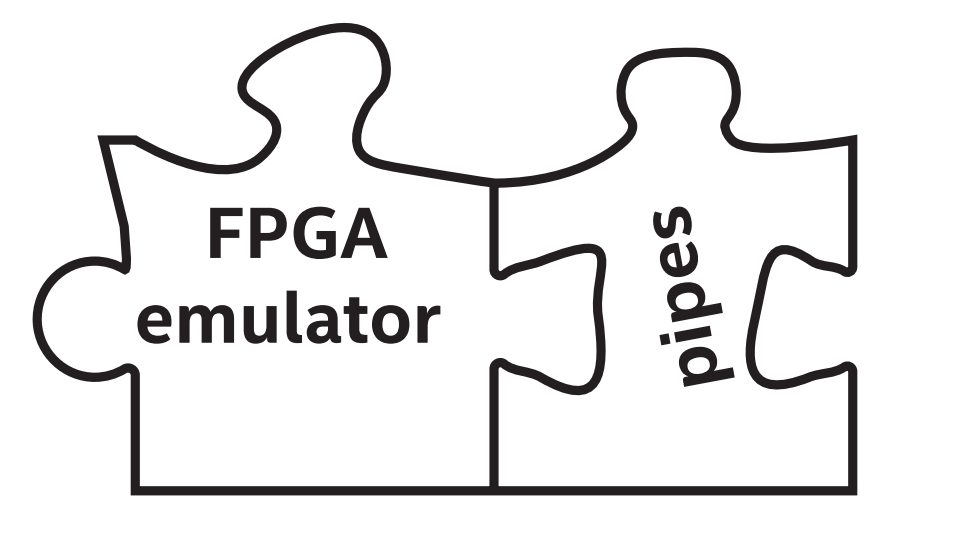
\includegraphics[width=0.5\textwidth]{content/chapter-17/images/1}
\end{center}

基于内核的编程最初是作为一种访问GPU的方式而流行起来的。由于现在已经在许多加速器中得到了推广,理解编程风格如何影响代码到FPGA的映射非常重要。\par

对大多数软件开发人员来说,现场可编程门阵列(FPGA)并不熟悉,部分原因是大多数桌面计算机在典型的CPU和GPU之外没有FPGA。FPGA的确很值得了开发人员来了解,因为它在很多应用中都有优势。和其他加速器一样,也需要问同样的问题,比如“什么时候使用FPGA?”,“应用程序的哪些部分应该加载到FPGA?”,以及“如何编写在FPGA上表现良好的代码?”\par

本章为我们提供了开始回答这些问题的知识,至少可以确定我们对FPGA是否感兴趣,并知道哪些构造可用于实现性能。我们可以阅读供应商文档来了解特定产品和工具链的详细信息。首先概述程序如何映射到FPGA等空间架构,然后讨论FPGA作为加速器的一些特性,最后介绍实现性能的编程结构。\par

本章的“如何使用FPGA”一节适用于任何FPGA。SYCL允许供应商指定CPU和GPU之外的设备,但没有具体说明如何支持FPGA。目前,对于特定的FPGA支持是DPC++的优势,即可以使用FPGA选择器和管道。FPGA选择器和管道是本章中使用的DPC++扩展。我们希望厂商能够使用类似或兼容的方式来支持FPGA,而DPC++作为一个开源项目非常鼓励这种做法。\par






















































